\subsection{VQ-GAN + CLIP Editing}
\begin{frame}[allowframebreaks]{Using CLIP for generative tasks}
    \begin{figure}
        \centering
        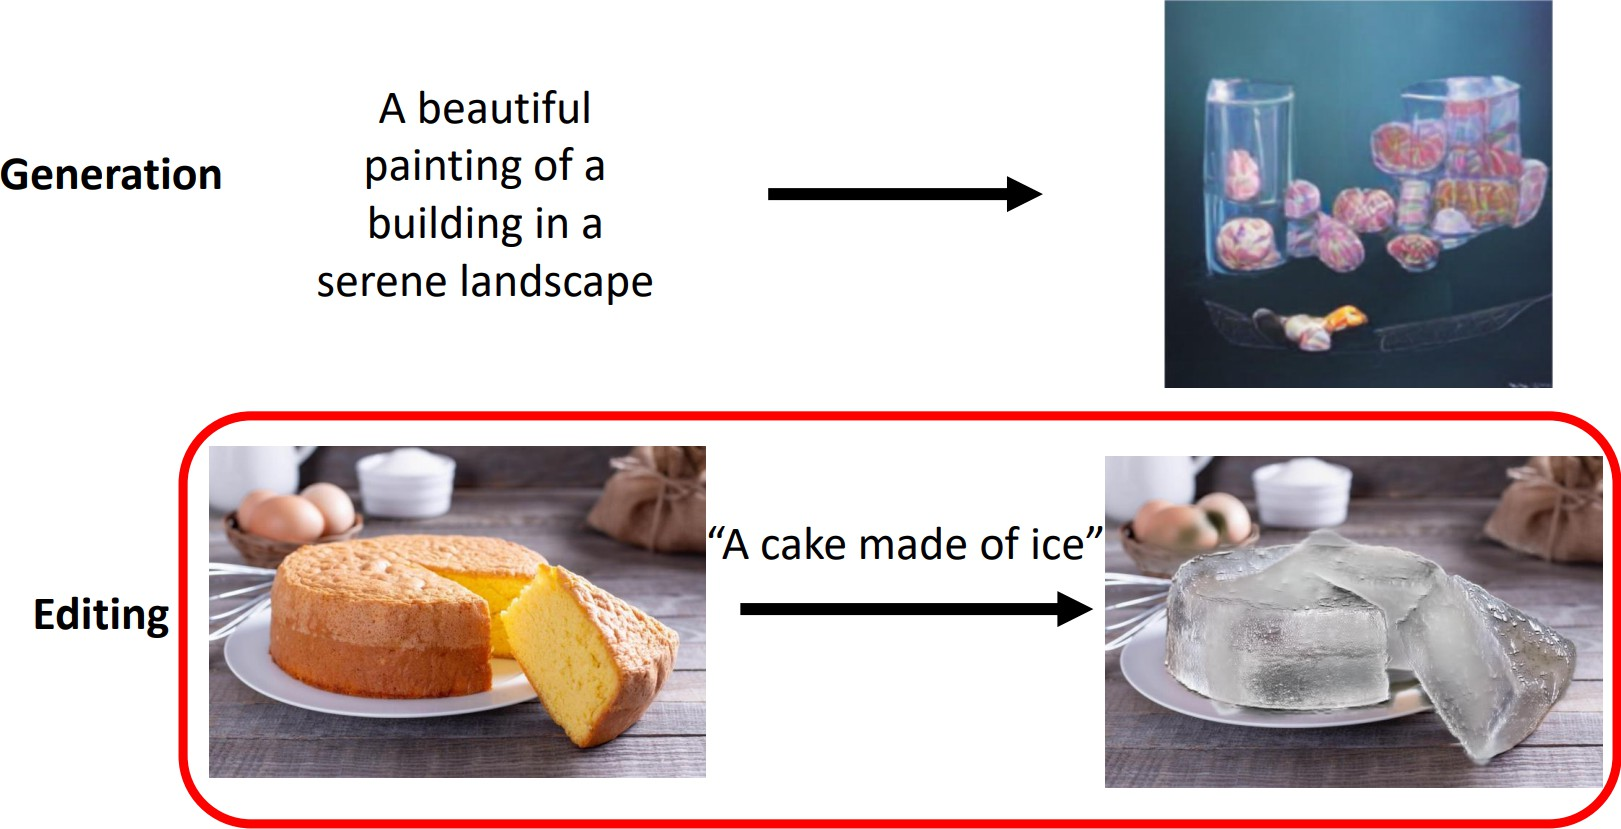
\includegraphics[width=1\textwidth,height=0.72\textheight,keepaspectratio]{images/video/slide_62_1_img.jpg}
    \end{figure}
    {\footnotesize{[Composite slide figure; generated image from VQGAN-CLIP, Crowson et al., ECCV 2022, Fig.~2]}}
\end{frame}


\begin{frame}[allowframebreaks]{VQ-GAN + CLIP Editing}
    \large Editing needs no new machinery: only the starting point changes. \\[1em]
    \normalsize
    \begin{itemize}
        \item \textbf{Initialization is the whole difference:} for generation the initial image is random pixel values; for editing it is the image we want to modify. The architecture and the loss are unchanged.
        \item \textbf{The prompt is used identically:} the text describing the desired change enters the CLIP similarity loss exactly as a generation prompt would.
        \item \textbf{Structure is retained} because the optimization starts from the source image. Where a region must be held fixed, the gradients on the corresponding parts of the latent vector can be zeroed out (masking).
        \item \textbf{Applications:} recolouring, weather and texture changes, and style transfer on real photographs, not only synthesis from scratch.
    \end{itemize}
    \vspace{0.5em}
    {\footnotesize{[VQGAN-CLIP, Crowson et al., ECCV 2022, Sections 2.5 and 4]}}
\framebreak
    \begin{figure}
        \centering
        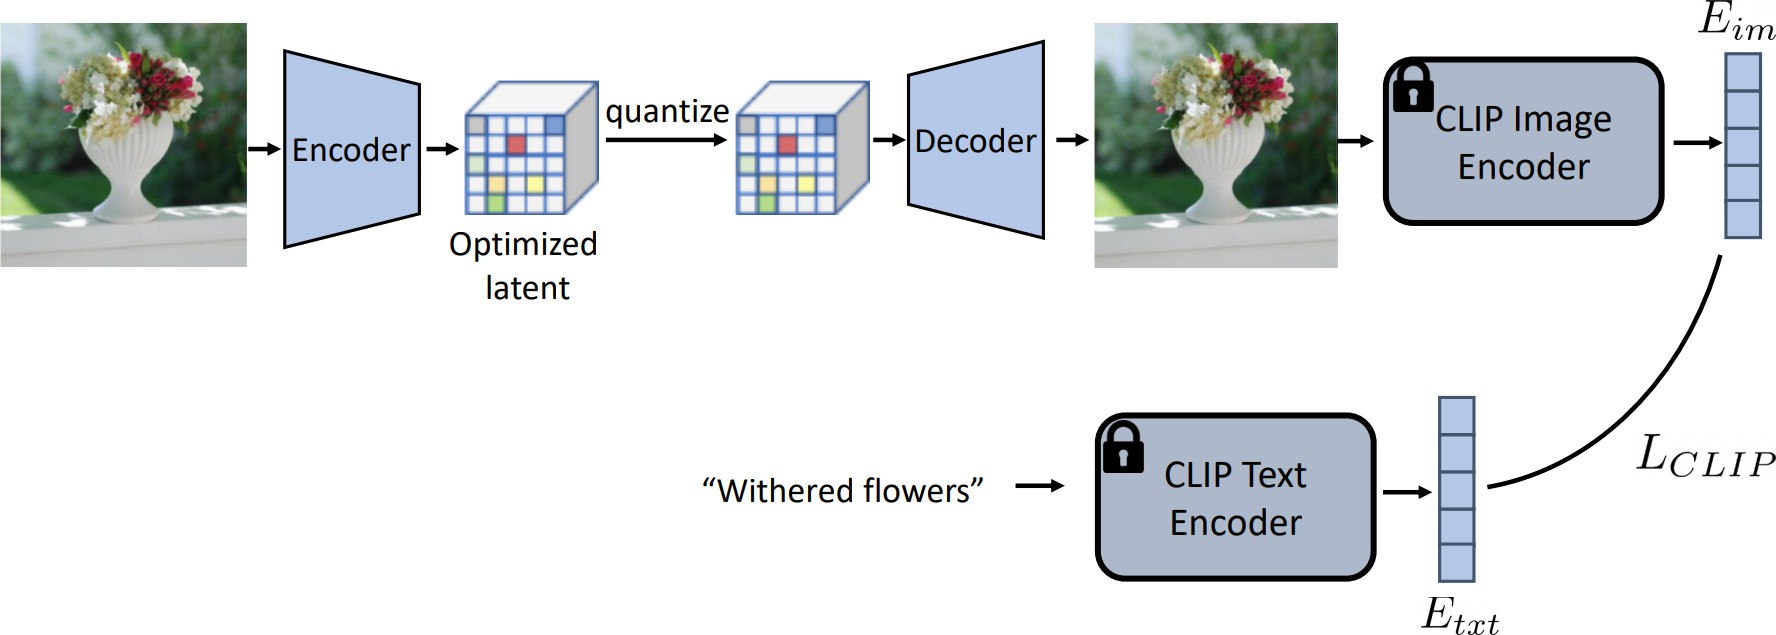
\includegraphics[width=1\textwidth,height=0.8\textheight,keepaspectratio]{images/video/slide_63_1_img.jpg}
    \end{figure}
    {\footnotesize{[VQGAN-CLIP: Open Domain Image Generation and Editing with Natural Language Guidance, Crowson et al., ECCV 2022]}}
\framebreak
    \begin{figure}
        \centering
        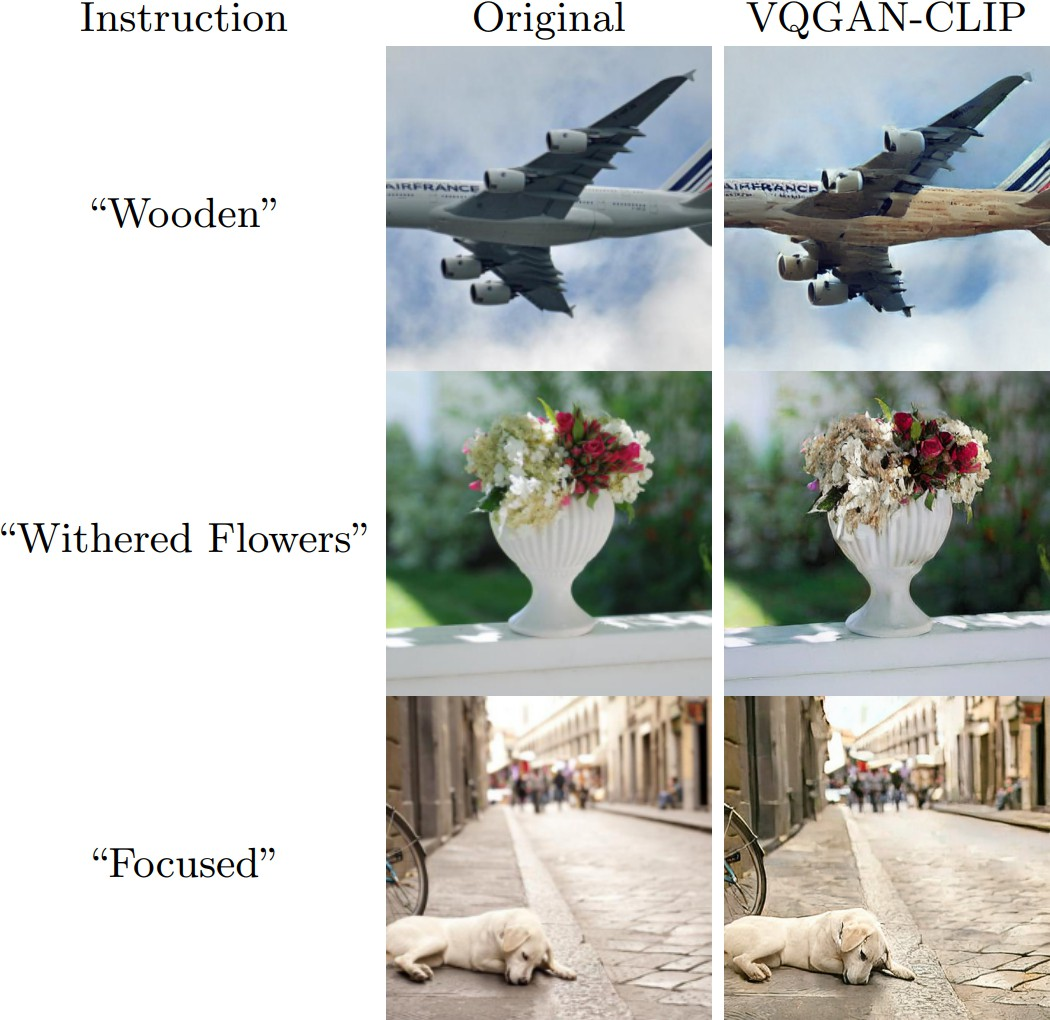
\includegraphics[width=1\textwidth,height=0.72\textheight,keepaspectratio]{images/video/slide_64_1_img.jpg}
    \end{figure}
    {\footnotesize{[VQGAN-CLIP: Open Domain Image Generation and Editing with Natural Language Guidance, Crowson et al., ECCV 2022, Fig.~7]}}
\end{frame}